%%%%%%%%%%%%%%%%%%%%%%%%%%%%%%%%%%%%%%
% Jordan Moak's Resume				 %
% Date: 10/22/2017					 %
% Type: Software QA					 %
%%%%%%%%%%%%%%%%%%%%%%%%%%%%%%%%%%%%%%

%!TEX TS-program = xelatex
\documentclass[]{moak-resume}

% Packages
\usepackage{afterpage}
\usepackage{hyperref}
\usepackage{color}
\usepackage{xcolor}
\usepackage{smartdiagram}
\usepackage{fontspec}
\usepackage{metalogo}
\usepackage[utf8]{inputenc}
\usepackage{tikz}
\usetikzlibrary{mindmap,shadows}
\usepackage{pgf-pie}
\usepackage{pstricks}


% Document Meta information.
\hypersetup{
    pdftitle={Jordan Moak's Resume},
    pdfauthor={Jordan Moak},
    pdfsubject={Resume},
    pdfkeywords={The Best},
    colorlinks=false,           % no link border color
    allbordercolors=white       % white border color for all
}


\begin{document}
\header{Jordan}{Moak}
      {Statistical Programmer / Software QA Engineer / Lifelong Reds Fan}
      

% In the aside, each new line forces a line break
\begin{aside}
%  
\includegraphics[scale=0.34]{img/circleme3.png}
  \section{Address}
    14003 Avalon E. Drive
    Fishers, IN
    ~
  \section{Phone}
    +513 417 4499
    ~
  \section{Email}
    \href{mailto:jordan.moak@gmail.com}{\textbf{jordan.moak@}\\gmail.com}
    ~
  % use  \hspace{} or \vspace{} to change bubble size, if needed
  \section{Programming}
	\programmingPie{}
	%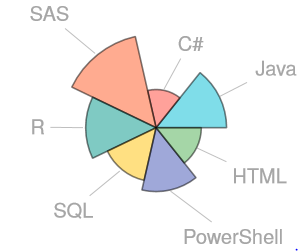
\includegraphics[scale=0.6]{img/progChart.png}
    ~
  \section{Future Interest}
    \textbf{R}
\includegraphics[scale=0.40]{img/5stars.png}
    \textbf{Java}
\includegraphics[scale=0.40]{img/5stars.png}
    \textbf{SQL}
\includegraphics[scale=0.40]{img/4stars.png}
    \textbf{Python}
\includegraphics[scale=0.40]{img/4stars.png}
    \textbf{Selenium}
\includegraphics[scale=0.40]{img/3stars.png}
    \textbf{Appium}
\includegraphics[scale=0.40]{img/3stars.png}
    \textbf{C Sharp}
\includegraphics[scale=0.40]{img/3stars.png}
    \textbf{SAS}
\includegraphics[scale=0.40]{img/2stars.png}
    %\textbf{PHP}
\includegraphics[scale=0.40]{img/1stars.png}
    ~
  \section{Personal Skills}
    \smartdiagram[bubble diagram]{
        \textbf{Problem}\\\textbf{Solving},
        \textbf{Initiative},
        \textbf{Curiosity},
        \textbf{Compe-}\\\textbf{tetive},
        \textbf{Leader-}\\\textbf{ship},
        \textbf{Efficiency}
    }
    ~
\end{aside}
~
\section{ \newline Summary}
\begin{entrylist}
	\entry
	{}
	{}
	{}
	{Dedicated, enthusiastic, and passionate programmer with experience in the statistical analysis and testing automation associated with medical device QA and clinical trials.  Driven by the prospect of exceeding expectations in the confrontation of challenging projects and responsibilities which expand personal skills, knowledge, and problem-solving ability.  Ambitious indiviudal offering a combination of exceptional motivation and a great logical sense to ensure the completion of projects ahead of expected timelines.\\}
\end{entrylist}
\\
\section{Experience}
\begin{entrylist}
  \entry
    {09/14 - Now}
    {DV Software Engineer}
    {Roche Diagnostics (Contracted through PRO Unlimited)}
    {Work both within a team and independently to write tools and test cases in order to verify the functionality of statistical and tracking applications in web portal and mobile application environments. Validate the processes and statistical analyses of software applications developed in the SAS BI development environment in regards to system requirements. Ensure mobile phones meet specifications and requirements within an application-device-web system.
    	\begin{itemize}
    		\item Continuously written a reusable suite of tools using a combination of Java, Selenium, Powershell, and SAS to both automate and simplify the effort necessary to validate software within standard processes.
    		\item Independently develop SAS programs to conduct statistical analyses and create output for verification of software operations, following system specifications and requirements documents.
    		\item Lead and operate within a team to create test scenarios and generate the associated datasets and input parameter files to ensure proper functionality of software applications.
    		\item Investigate malfunctions and discrepancies in order to provide detailed feedback and offer solutions to software developers.
    	\end{itemize}}
  \entry
    {03/14 - 08/14}
    {Programmer/Analyst}
    {The Stevenson Company}
    {Operated as a member of an IT/development team to produce, maintain, and update statistical web applications and tools for market research. Developed statistical procedures to conduct quality control analyses and clean new data entering the system.
    	\begin{itemize} 
    		\item Implemented programs to systematically clean data and produce statistical output for data monitoring.
     		\item Evaluated existing methods of data processing to improve efficiency and code readability, as well as converting existing SAS programs into MySQL and PHP.
     		\item Investigated anomalous occurrences and statistical trends to provide feedback to clients.
     		\item Executed and reviewed methods to produce accurate market sizing calculations.
    	\end{itemize}}
\end{entrylist}
\\
\newpage
\section{More Experience}
\begin{entrylist}
    \entry
    {01/13 - 12/13}
    {Statistical Programmer}
    {STATKING Clinical Services}
    {Collaborated within a programming team to complete data management and statistical analysis of 20+ phase I, II, and III clinical trials in various therapeutic areas. Developed CDISC standard SDTM and ADaM submission datasets using the SAS programming language. Produced SAS programs to generate safety and efficacy tables, listings, and figures.
    	\begin{itemize}
    		\item Lead the production of 160+ tables for a Phase III Clinical Trial.
    		\item Designed SAS programs as tools to complete common tasks more efficiently.
    		\item Operated in accordance with standard operating procedures (SOPs) to ensure the employment of good clinical practices.
    		\item Authored and executed Data Management Plans, Program Design Documents, Logic Checks, Test Plans, and Test Plan Summary Reports.
    		\item Created data entry screens and edit check validations using electronic data capture software.
    	\end{itemize}}
    \entry
    {01/08 - 06/08}
    {Intern/Student Teacher (Mathematics)}
    {Little Miami Junior High}
    {Assisted in class instruction and maintaining productive and enjoyable work environment for students. Created keys, recorded and maintained records for student assessment, and reviewed lesson plans to ensure accordance with state education regulations. Tutored students individually to better solidify understanding of the material.}
\end{entrylist}
\\
 \section{Programming Packages}
 \begin{entrylist}
 	\entry
 	 {\textbf{ SAS}}
 	 {\textnormal{SAS-Macro, SAS BI, SAS ODS, SAS Graphics, PROC Report, PROC SQL, PROC Tabulate, PROC IML}}
 	 {}
 	 {}
 	\entry
 	 {\textbf{Java}}
 	 {\textnormal{JUnit, Selenium, Appium, JSoup, Swing}}
 	 {}
 	 {}
 	\entry
 	 {\textbf{     R}}
 	 {\textnormal{RPostGresSQL, RSQLite, multcomp, ggplot2}}
 	 {}
 	 {}
 \end{entrylist}
\\
\section{Education}
\begin{entrylist}
  \entry
    {2008 - 2013}
    {Bachelor's Degree in Mathematics}
    {Northern Kentucky University}
    {Specialization in Applied Mathematics\\}
  \entry
    {2008 - 2013}
    {Bachelor's Degree in Statistics}
    {Northern Kentucky University}
    {Capstone project written in the R programming language to detect anomalies in credit card usage data, then predict the legitimacy of such detections as occurrences of fraudulent behavior.\\}
\end{entrylist}
\\
\footer {References \& Code Samples Available Upon Request}
\end{document}
